\documentclass[12pt]{article}
\usepackage{braket}
\usepackage{physics}
\usepackage{graphicx}
\usepackage{times}
\usepackage[export]{adjustbox}
\usepackage{listings}
\usepackage{mathcomp}
\usepackage{hyperref}
\usepackage{bm,amsmath}
\usepackage{float}
\usepackage{indentfirst}
\usepackage{bigints}
\usepackage{amssymb}
\usepackage{mathtools}
\numberwithin{equation}{section}
\title{Particle Net Paper}
\author{Ting-Kai Hsu}
\date{Sep}

\begin{document}
\maketitle
\tableofcontents

\section{Introduction}
This document is for some important points in \textit{H.Qu and L.Gouskos, Jet Tagging via Particle Clouds}.
When we would like to study experimental pariticle physics, finding the origin particles initializing the jets(a lot of quarks) is an important skill. For instance, jets initialed by gluons tend to have a boarder energy spread than the jets initialed by quarks.High-momentum heavy particles would have jets with multi-prong structure. A tranditional way to organizing jets is to put them into ordered structure(like tree or sequence) based on their constituent particles. In this paper, they introduce a novel way, that is, treating the jets as \textit{unordered} particles, or called \textit{particle cloud}.
\\
\indent The technique of indentifying the particle heavily relies on the representation of jets, the paper would go through some classical representations and then introduce theirs. 

\section{Imaged-Based Representation}
\textit{ref: }\href{https://link.springer.com/article/10.1007/JHEP02(2014)057}{ResNet}   \href{https://ieeexplore.ieee.org/document/7780677}{Inception}
\\
\indent This representation origins from the measurement of the energy of particles by \textit{calorimeter}. The calorimeter would measure the enregy deposition of a jet and then reconstruct the spatial distribution of jet pixel by pixel. It could improve the performance.
\\
\indent However, there are 2 main shortcomings with this representation.

\begin{itemize}
    \item It would include all information measured by calorimeter; however, it is difficult to adding additional properties of jet if we want to fruit the information of a certain jet, and it is a problem to put additional information into the cell.
    \item Treating jet as \textit{image} would also lead to a very \textit{sparse} representation. Typically, we would need $\mathcal{O}(1000)$ pixels to represent a jet containing $\mathcal{O}(10) \sim \mathcal{O}(100)$ particles, which make the calculation very \textit{inefficient}. 
\end{itemize}

\section{Particle-Based Representation}

This may be the natural way to represent the jet, that is, we veiw the jet as the collection of its constituent particles. This representation allows us to include all features of particles, which makes it more flexible than image representation. Moreover, it has a much more compact form for storing information than image representation, though the length of different jets would vary since they contain different number of particles. The collection of particles would be \textit{sequence} in practice. Also, there should be a storing mathod to assign the position of each element, for instance, storing them in sequence according to their transverse momentum. Another way of realizing the particle-based representation is using the \textit{binary tree} based on $QCD$ theory. The shortcoming of this representation would be the \textit{non-intrinsic} order of constituent particles of jet, which requires manual operation on informaiton to order and store the particle into sequence and tree, and turns out to impair the performance.

\section{Jet As Particle Clouds}

In this section, we would go through the new way in this paper. It says that a more natural representation for a jet would be an \textit{unordered, permutation invariant\footnote{also called \textbf{permutation symmetry}, this is a property of a mathmetical funciton or an algorithm that remain unchanged even if the position or the order of the elements is altered. \href{https://medium.com/@he165076373/what-is-permutation-invariance-a-brief-introduction-58ecb7a49334}{\textit{ref.}}, Which means we are able to put the inputs into container without ordering them as in image representatoin.}} set of particles. It shares the properties of the particle-based representation, which allows to include the features and additional information of particles if we want. The paper points out this notion is related to a type of method storing data in computer vision, that is, \href{https://en.wikipedia.org/wiki/Point_cloud}{\textit{point cloud}}, which is also an \textit{unordered} set storing the position distribution irregularly in space.\footnote{there are several reason, first is that the detector starts scanning randomly. Second is for efficiency and flexibility and reduciton of information.} Even though we say the storagement would be unordered, this doesn't mean there isn't any relaiton between the points or particles, but they do have some internal connection since they represent higher-level object(jet). This isn't a new idea though, and the paper points out that the old way \href{chrome-extension://efaidnbmnnnibpcajpcglclefindmkaj/https://arxiv.org/pdf/1810.05165.pdf}{Energy Flow Network} doesn't put emphasis on the spatial structure of particles.

\section{ParticleNet Implementation}

In this section, we would introduce ParticleNet, a \textit{CNN-like} deep neural network for jet tagging with particle cloud data. First, we should go through two key features of \textit{Convolution Neural Network, CNN}. 

\begin{itemize}
    \item the convolution operation exploits translational symmetry\footnote{ In natural images, objects or features often appear in different parts of the image but share the same characteristics. For example, a cat's face can appear anywhere in an image, and the patterns that make up the cat's face are the same regardless of its position. This is known as translational symmetry.} of images by using shared kernels across the whole image, which is a way to reduce the number of parameters and meanwhile enhance the efficiency.
    \item Hierarchical approach in deep learning splits the funcitons of learning into different layers, for deeper layers, they should study for the more general patterns, and for the shallower layers, they should focus on local information. CNN can learn features at different scales by hierarchical approach.
\end{itemize}

We could adopt similar method like CNN to represent the point cloud; however, there are some differences making regular convulotion difficult to be applied on point-cloud representation. One main reason is that in the point-cloud representation, we've expected that the particles would distribute irregularly within the space. Also, we know that the regular convolution wouldn't be invariant under permutation, so we need to carry out a similar method with some modification. Recently, there is a method called \href{chrome-extension://efaidnbmnnnibpcajpcglclefindmkaj/https://dl.acm.org/doi/pdf/10.1145/3326362}{edge convolution \textit{EdgeConv}}. This method starts setting the points themselves on the vertices, treating them as graph, and setting the edges to be the connections of point to its $k$ nearest neighboring points. As mentioned in Deeping Learning, the \textit{local patch} here is defined as the $k$ nearest neighboring points. 
\\
\indent Here we're going through the edge convulotion. We compute a directed graph $\mathcal{G} = \left(\mathcal{V}, \mathcal{E}\right)$ representing local point cloud structure, where vertices $\mathcal{V} = \left\{1, \hdots, n\right\}$ and edges $\mathcal{E} \subseteq \mathcal{V} \times \mathcal{V}$. By above description, we construct graph as the nearest $k$ neighbor ($k$-NN) graph of $\mathbf{X}$ in $\mathbb{R}^F$, where $F$ is the dimension. The graph includes \textit{self-loop}, meaning each node also points to itself. We define \textit{edge features}\footnote{that can represent edges} as $\pmb{e}_{ij} = h_{\pmb{\Theta}}(\mathbf{x}_i, \mathbf{x}_j)$ where $h_{\pmb{\Theta}}$ is a nonlinear function with a set of \textit{learnable parameters} $\pmb{\Theta}$. Then we apply a \textit{channel-wise symmetry}\footnote{this is a property of filters(or called kernels) which mean the kernels exhibit symmetry across the channel. It is the key property used for the networks demanding permutation symmetry.} aggregation operation $\Box$ (like $\sum$ \textit{sum-pooling} and $\max$ \textit{max-pooling}). This operation would be used on \textit{edge features} associated with all edge coming from each vertix. The output would be a new point that could be represented by the orginal representation.

\begin{equation}
    \mathbf{x}'_i = \mathop{\square}_{j:(i, j) \in \mathcal{E}} \pmb{e}_{ij} = \mathop{\square}_{j:(i, j) \in \mathcal{E}}h_{\pmb{\Theta}}(\mathbf{x}_i, \mathbf{x}_j)
\end{equation}

But it seems confusing for the meaning of $\mathbf{x}_i$ and $\mathbf{x}_j$, and we make analogy to the regular convolution. $\mathbf{x}_i$ would be the center vertex while kernel is applied on the inputs, and $\mathbf{x}_j$ would be the vertices surrounding to it.

\begin{figure}[H]
    \centering
    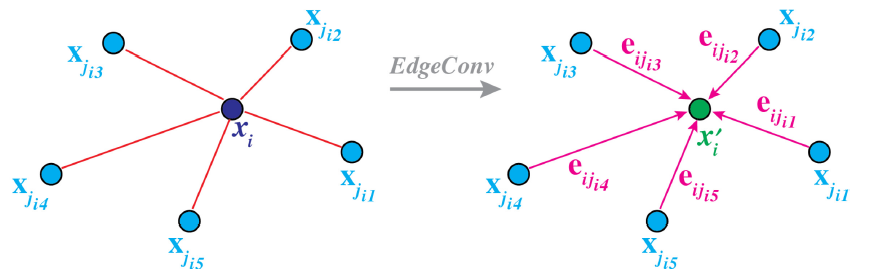
\includegraphics[width=0.75\linewidth]{x_ix_j.png}
    \caption{Relation of $x_i$ and $x_j$}
    \label{1}
\end{figure}

To sum up, for $F$-dimensional point cloud, EdgeConv would produce a $F'$-dimensional point cloud with the same number of points. \textit{The choice of edge function $h_{\pmb{\Theta}}$ and aggregation funciton $\square$ would have critical influence.}
\\
\indent \textit{\textbf{Example 1:} for $\mathbf{x}_1, \hdots, \mathbf{x}_n$ representing the image pixels, and the graph $\mathcal{G}$ has the connectivity representing patch fo fixed size around each pixel $\mathbf{x}$.} Choosing \[h_{\pmb{\Theta}}(\mathbf{x}_i, \mathbf{x}_j) = {\pmb{\theta}_m}\cdot\mathbf{x}_j\], where $\pmb{\Theta} = \left\{\pmb{\theta}_1, \hdots, \pmb{\theta}_M\right\}$ is the learning variables representing for the weight of $M$ learning layers(filters).
And by choosing the aggregation function to be the summation

\begin{equation}
    x_{im}' = \sum_{j: (i, j) \in \mathcal{E}}{\pmb{\theta}_m \cdot \mathbf{x}_j}
\end{equation}

As we all know, this is simply the regular convolution. 
\\
\indent They use the same method designed for point cloud on the ParticleNet, where the edge function, which is a \textit{asymmetric} function, would be defined as below,

\begin{equation}
    h_{\pmb{\Theta}}(\mathbf{x}_i, \mathbf{x}_j) = \bar{h}_{\pmb{\Theta}}(\mathbf{x}_i, \mathbf{x}_j - \mathbf{x}_i)
\end{equation}
As we could know from above, if we change the order of $\mathbf{x}_i$ and $\mathbf{x}_j$, the function on RHS would look different. Explicitly, we'd have the edge function look like,

\begin{equation}
    \bar{h}_{\pmb{\Theta}}(\mathbf{x}_i, \mathbf{x}_j-\mathbf{x}_i) = e'_{ijm} = \text{ReLU}\left(\pmb{\theta}_m\cdot\left(\mathbf{x}_j-\mathbf{x}_i\right)+\pmb{\phi}_m\cdot\mathbf{x}_i\right)
\end{equation}

where $\pmb{\theta}_m, \pmb{\phi}_m$ are the learning variables $\pmb{\Theta}$ and the function ReLU simply elimanating the negative result.

\[ \text{ReLU}(x) = \max(0, x) \]\footnote{why we use ReLU but not the other \textit{activation functions} is that we would like to impose the physical meaning on the edge features, that is, it shouldn't be negative since it represents the edge between the points.}

In 5.4, the global shape would be captured by the coordinates of the patch centering $\mathbf{x}_i$, and the local structure would be captured by $\mathbf{x}_j - \mathbf{x}_i$. And the aggregation function $\square$ would be maximum, that is,

\begin{equation}
    \mathbf{x}'_{i} = \mathop{\max}_{j: (i, j) \in \mathcal{E}}e'_{ijm}
\end{equation}

Because $\max$ is a \textit{symmetric function}, we could say this method is \textit{permutation invariant}.
\\
\indent \textit{\textbf{Partial Translation Invariant: }if we consider a shifting $\pmb{T}$, then we can show that partial information would be preserved by this translation.}

\[ e'_{ijm} = \text{ReLU}\left(\pmb{\theta}_m\cdot(\mathbf{x}_i+\pmb{T}-\mathbf{x}_j-\pmb{T})+\pmb{\phi}_m\cdot\left(\mathbf{x}_i+\pmb{T}\right)\right) \]
\[ = \text{ReLU}\left(\pmb{\theta}_m(\mathbf{x}_j-\mathbf{x}_i)+\pmb{\phi}_m\cdot\left(\mathbf{x}_i+\pmb{T}\right)\right)\]

When we can see if $\pmb{\phi}_m = 0$, the edge funciton would be \textit{totally transation invariant}. However, if so we will lose the global information. However, the aggregation function chosed in this paper of particle cloud is different from that of the paper of point cloud, that is, they chosed the aggregation funciton to be \textbf{mean} $\frac{1}{k}\sum$. As we've mentioned before, EdgeConv can be seen as the mapping from the original point cloud to another new point cloud with the same number of points, that is, we can \textit{stack the layers} and operate EdgeConv one after another. The key property not only allow us to learn the features of particle hierarchically but also 
allows the position of points to be dynamically learnt by EdgeConv operation.
\\\\
\indent After introducing the original approach in paper of point cloud, however, we should remark some differences between it and the method used in this paper for particle cloud. Below would be our general EdgeConv block,

\begin{figure}[H]
    \centering
    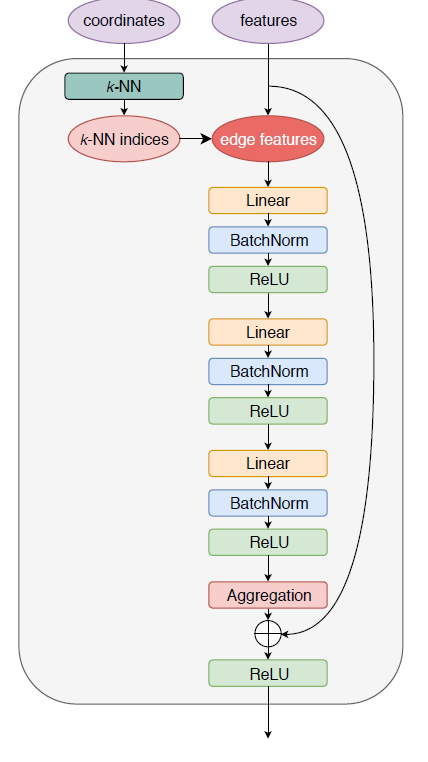
\includegraphics[width=0.35\linewidth]{The Structure of the EdgeConv block.png}
    \caption{The Structure of the EdgeConv Block}
    \label{2}
\end{figure}

In Figure 2, we can see that there would be 2 inputs, first the operation would start with the "\textit{coordinates}" input, and using them to compute the distances to find the $k$ nearest neighbors. Then the $k$-NN($k$ nearest neighbor) indices, along with the "\textit{features}" inputs, would be sent to EdgeConv operation. A shortcut running parallel to EdgeConv is implemented, allowing the "\textit{features}" inputs to pass through directly. There are three layers \footnote{The number of layers in implementation is determined by experiment.}
and each layer contains a linear transformation, followed by \textit{batch normalization}\footnote{This is a method that can enhance the efficiency by normalizing the inputs before every operation. Letting the data distribution to be $\mu = 0, \sigma = 1$ normal distribution. And often before the activation and after the linear transformation. Precisely, Batch normalization helps networks converge faster during training, reduces the sensitivity to the initialization of weights, acts as a form of regularization, and allows for the use of higher learning rates.}, and then the rectified linear unit function(ReLU). There are two hyperparameters in each EdgeConv block, and one is the $k$ nearest neighbors, and the other one is the channels $C = (C_1, C_2, C_3)$\footnote{The number of channels represents the units or storage used in the layer.}.\\
\indent Then the ParticleNet architecture would be as following,

\begin{figure}[H]
    \centering
    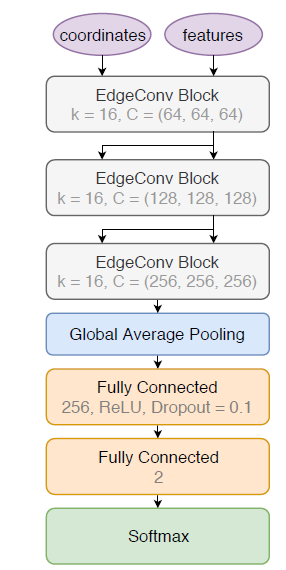
\includegraphics[width=0.35\linewidth]{ParticleNet.png}
    \caption{ParticleNet Architecture}
    \label{3}
\end{figure}

which contains 3 EdgeConv block, each filtering different features. The number of channels are \textit{increasing} because the amount of informaiton is going up and need more storagements. Following is the \textit{Global Average Pooling}. this is applied because the average pooling in each EdgeConv layer would only aggregate the feature they would looking for, and we need to aggregate globally all the learnt features all over the particles in the cloud. And then we go to the \textit{Fully Connected} layer\footnote{or \textit{Dense layer}}. And why we need fully connected layer, because it is fully connected to the previous layers and the following layers and its neurons are connected to others.This helps the model to learn some intricate patterns and relationship. And it may be able to learn the features of the features inputed from the previous layers.\footnote{Fully connected layer is often put in the top of each other in the hierarchical structure is because it can afford more complicated information.}
\\
\indent Also in the first dense layer, we have a special funciton that is designed to afford the \textit{overfitting} when training data, that is, \textit{dropout function}. What the dropout function is that it intentially to discard some input data when training data. This is along with the \textit{dropout pobability} which represents how much training data the model should discard. And then we go on to another dense layer. Finally, we meet a special function \textit{softmax function}.
It works at the output layer, and turning the data from the previous layer into \textit{probability};however, the transformation is not that simply \[p_i = \frac{s_i}{\sum_{j}s_j}\], rather we take \[p_i = \frac{e^{s_i}}{\sum_{j}e^{s_j}}\] for some \href{https://www.youtube.com/watch?v=8ps_JEW42xs}{reasons}. Therefore, it simply means the procedure of ParticleNet would turn the features into probability distribution.

\section{Performance-Top Tagging}

After introducing the core concept and the implementation of ParticleNet, we're going to show some results and performance in this paper with the novel method. For starters, we go through the classical "\textit{top tagging}"\footnote{Identifying the jets coming from top quarks \textit{hadronic} decation.}. As in the final goal of the tutorial I has studied for the $t\bar{t}$ reaction, t-tagging acts an important role.
There are some requirement that the jet should meet if it is included in the process, mostly associated with the angular distribution of jets.
\footnote{$\eta$ stands for the angle in pseudorapidity between the particle and jet-axis. And $\phi$ stands for the angle in azimuthal angle between the particle and the jet axis.}
\\\indent
Before going into EdgeConv, we need determine how many variables we need to use. 

\begin{itemize}
    \item $\Delta \eta$ As we mention before, it is the difference of the angle in pseudorapidity.
    \item $\Delta \phi$ Similarly, these 2 parameters would be taken to calculate the distance of particles.
    \item $\Delta R = \sqrt{\Delta \eta ^2 + \Delta \phi ^2}$
    \item $\left(p_x, p_y, p_z, E\right)$ We only consider some particles with highest of these quantities. 
    \item $\log(p_T) \text{ and } \log(E)$
    \item And their relative amount with respect to jet, $\log(\frac{p_T}{p_{T, jet}})\text{ and }\log(\frac{E}{E_{jet}})$
    \item The charge the particle brings, $q$
\end{itemize}

These quantities would be taken as \textit{input features}. When comparing the performance with other models, the paper mentioned another similar way that also storing the information in \textit{unordered set}, but it only consider the global structure but ignore the local neighboring information, and this method is called \href{https://arxiv.org/abs/1810.05165}{Particle Jets}. Some \textit{background rejection metrics} have improved rapidly in ParticleNet. For instance, the background rejection $\frac{1}{\epsilon_{B}}$ is lower with given signal efficiency $\epsilon_{S}$.

\section{Performance-Quark Gluon Tagging}

The interaction between quarks and gluons makes it difficult for us to seperate and identify them, that is, the quark gluon tagging works for seperating the signal(quark) from the background(gluon), and discriminates the jets initialized by quarks and by gluons. In this paper, they dealt with the process \[ Z^0 \left(\rightarrow \nu\nu\right) + (u, d, s) \] and \[ Z^0 \left(\rightarrow \nu\nu\right) + g \]
In this case, only transverse momentum $p_T$ between certain range and \textit{rapidity}\footnote{Rapidity is a measurement that is invariant and measures how fast is a velocity of a motion reaches to light speed. \href{https://en.wikipedia.org/wiki/Rapidity}{\textit{ref}}} $\abs{y}$ above certain value are considered. More amount of information are in consideration in EdgeConv in quark-gluon tagging that in top tagging, and precisely, the identity of particle(photon, electron, pion, and so on) is included. Here we only consider five types of particle,

\begin{itemize}
    \item Electron
    \item Photon
    \item Muon
    \item Charged Hadron 
    \item Neutural Hadron 
\end{itemize}

The result shows the power of particle cloud and particle jets because they can add the information of particles, like the identity of them, which helps a lot.

\section{Model Complexity}

In this section, we're going to show the complexity of ParticleNet, that is, we'll show the number of parameters and the computational cost. Here we should notice that the computational cost is represented by the \textit{inference time}\footnote{Inference time specifically refers to the time it takes for a machine learning model to make predictions or inferences on new, unseen data. It measures the computational cost of processing a single input through the model to obtain a prediction.}
 but not the real-life running time when training the data.

\section{Conclusion}

Finally, the paper emphasizes that deeper architectures can generally lead to
better performance.
\\
\indent \textbf{Applications
of the particle cloud approach to, e.g., pileup identica-
tion, jet grooming, jet energy calibration, etc., would be
particularly interesting and worth further investigation.}
\end{document} 